\chapter{Network State Modeling using Sparse Clustering Autoencoders}
	\label{cha:sparse_clust}
	   	
   	Unsupervised learning can be utilized as an	exploratory tool for data mining, as an initial approach in case of new contexts and unknown datasets, such as when developing an applications that uses deep learning algorithms.
   	Associating observations with each other, i.e. the discovery of existing groups in the data based on meaningful similarity, is one of the most powerful tools for such uses.
   	Association can be undertaken through the \ac{ML} task of clustering, the most often utilized subcategory of unsupervised learning.   	
   	Clustering can be a very complex task, as it relies heavily on the understanding of the latent behavior, the underlying causes in the data.
   	
   	Clusters are often subjective, because the ground truth is up to interpretation, however contradictory this might sound: where one might see a feature which clearly separates two groups with barely any points in-between, another could say that there are enough transitional observations so that the two groups cannot be separated.
   	Furthermore, taking only a few features into account might separate the observations into a few clusters, while including more features could split the data into more clusters.
   	It is up to the individual to define what ``meaningful'' is in a certain setting.
   	
   	While the above is mostly true for clustering natural behavior, such as the behavior of humans, clustering in artificial systems can be a little more well-defined.
   	In artificial systems -- such as mobile networks -- the use of clustering is usually tied to a problem or a task to solve, which can immediately designate the features that are meaningful for the clustering.
   	Furthermore, artificial systems often have state-like logic, forming clusters in the behavior which are objectively true, and not up to interpretation.
   	Naturally, these clearly defined groups are often tied to-, or influenced by less clearly defined behavior, such as human interaction with the system.
   	In any case, the true cause of behavior is often hidden, and can only be extracted through the understanding of the latent logic in the data. 	
   	Thus, in our nomenclature, clustering is more than just simple grouping; clustering requires understanding of the underlying logic in the data, so that clusters may be formed not on superficial, surface-level features, but deep and meaningful connections between the observations.
   	This need for a better understanding of the data leads to the idea of realizing clustering using deep learning.
   	
	Clustering shares mechanical similarities to quantization; both tasks define groups based on training observations.
	Where we distinguish the two is in the end goal; quantization aims to split the training data -- thus the input space -- into many small quanta, without necessarily assigning existing groups or other ground truth to a single quantum.
	Opposite to this, clustering aims to find existing groups in the data, in a one-to-one mapping between \emphnox{ground truth classes} and \emphnox{formed clusters}.
	Because of the probably much more complex definitions (shapes) of clusters, generally clustering also does not aim to represent groups with singular observations (prototypes), unlike quantization.
	However, the distinction between quantization and clustering is not always so simple: as we have seen briefly in the end of the previous chapter, often the best approach to quantization is to recognize the existing groups in the data, thus employing some clustering techniques in the feature selection/quantization process.
	This chapter discusses an algorithm that is also somewhat in-between quantization and clustering, but approaches the problem from the other direction, by ``over''-partitioning space into many micro-clusters, and later connecting these to from actual clusters in the data.
	
	The core of the chapter is contained in Sec.~\ref{cha:sparse_clust:sec:sparse_ae}, which details the work published in the following paper:
	
	\begin{publication}
		Deep Clustering of Mobile Network Data with Sparse Autoencoders \\
		\textit{Márton Kajó, Benedek Schultz, Georg Carle} \\
		NOMS 2020-2020 IEEE/IFIP Network Operations and Management Symposium, pp. 1-6. IEEE, 2020.
	\end{publication}

	My contributions to the above paper was the design, implementation and evaluation of the algorithm, as well as the co-authoring of the paper.
	The discussion in this thesis expands on the paper, by adding further detail to some elements, as well as detailing the shortcomings of the algorithm in Sec.~\ref{cha:sparse_clust:sec:bias}.
	The algorithm discussed in this chapter is also contained in the following patent application:
	
	\begin{patent}
		Method and Apparatus for Automatic Network State Modeling in Mobile Networks using Deep Clustering Autoencoders \\
		\textit{Benedek Schultz, Márton Kajó, Stephen S. Mwanje} \\
		Finnish application no.: 20206162, filed November 2020
	\end{patent}

	The discussion is concluded with some remarks on design-time bias in algorithm design, and the caveats when designing \ac{DL} algorithms for explainability.

	\section{Deep Clustering with Sparse Clustering Autoencoders}
		\label{cha:sparse_clust:sec:sparse_ae}

		\subsection{State Transition Graphs, Sparsity of Activations}
			\label{cha:sparse_clust:sec:act_sparse}

			We have discussed network states previously in the context of facilitating communication between \acp{CF}.
			Network states describe the settings, performance, and/or context of single or multiple entities in the network, such as base-stations, gateways, cells, or users.
			Naturally, the network is not expected to always stay in the same state, rather, to often transition from one state to another.
			In this model, network elements exist in a shared state-space, where they are modeled as either being in a state, or moving from one state to another.
			Thus, the possible state-space can be envisioned as a network \emphix{state transition graph}{state transition graph}, where states are nodes, and transitions are connections running between these nodes.			
			An illustration of a network state transition graph can be seen in Fig.~\ref{fig:stategraph_transitions}.
			The graph allows for an easy overview of network behavior, as well as enabling simple graph-based solutions to a handful of use cases; anomaly detection, network state prediction, transfer learning of network state models, etc.
			
			Clustering is realized in the state transition graphs if we examine the population of transitions between the networks states.
			On one hand, populated transitions -- transitions which often see observations in-between two states -- signify a not so clear distinction between the states, which means that the states likely belong to the same ground truth group.
			On the other hand, unpopulated transitions show a clear division between two states, signifying separate ground truth groups.
			Populated and unpopulated transitions show up in a state transition graph as edges containing many or few observations.
			By only considering edges in the graph above a certain transitional population threshold, the state transition graph falls apart into disconnected subgraphs.
			The disconnected subgraphs form the clusters, where all network states are reachable from one another are considered as being in the same network state cluster.
			
			\begin{figure}[ht]
				\centering
				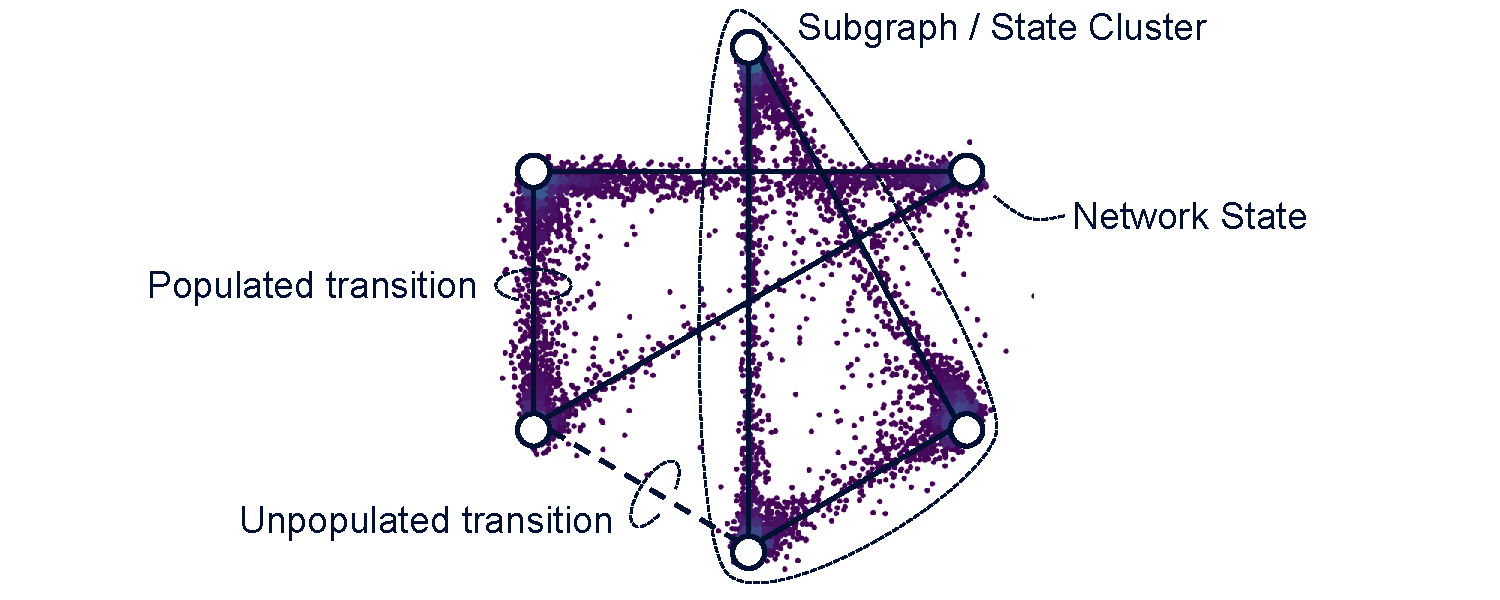
\includegraphics[width=\linewidth]{figures/06_sparse_clust/stategraph_transitions/stategraph_transitions.pdf}
				\caption[Network state transition graph illustration]{Illustration of a network state transition graph.}
				\label{fig:stategraph_transitions}
			\end{figure}
			
			The state transition graph concept is limited to linear transitions by design, where the network elements can only occupy transitional positions between $2$ states, i.e.: every observation is described either as a single state, or a mixture of $2$ states (as opposed to mixtures of $3$ or more states).
			This design decision was made for two reasons: 1) linear transitions are intuitive for us humans, because in a sense they represents movement from point $A$ to point $B$, and 2) they allow the model to be utilized as a graph.
			While the formulation of the states (nodes) in the graph could be done with previously described quantization methods, the correct mapping of transitional observations to graph edges is not a trivial task.
			For the formulation of the state transition graph, we have chosen to use an autoencoder.			
			For the correct mapping of the transitional states, soft constraints need to be enforced during the autoencoder training, which move the encoded points onto lines between the defined graph nodes.
			As the encoding is already restricted by this constraint, it is beneficial to also fix the graph nodes to certain points in the encoding space, which results in a simple geometrical shape and an easier calculation of the constraint.
			
			By fixing the graph nodes in place, and moving encoded observations close to these points, or onto the lines connecting them, we enforce \emphix{activation sparsity}{activation sparsity} in the autoencoder, which refers to the situation where only a few neuron outputs (activations) are non-zero for every observation in a neural net layer.
			Activation sparsity is not to be confused with sparsity in space, referencing parts of the input space which contain few observations (are sparsely populated).
			Because the formulation of the state transition graphs is done through this enforcement of activation sparsity, our algorithm is called \ac{SCA}.

		\subsection{Sparse Clustering Autoencoders}
			
			The clustering method proposed here is based on an autoencoder, as introduced in Sec.~\ref{cha:deep_learning:sec:ae}.
			In their original form, autoencoders are trained to perfectly reconstruct of observations without any additional labeled information.
			Perfect reconstruction is not trivial, as the autoencoder is forced by its own topology to encode the observations into a lower dimensional space, and has to reconstruct (decode) them from this simplified representation.
			During training, the autoencoder tries to minimize a \emphnox{reconstruction loss}, measured in the data-space between the original and the reconstructed observations.
			
			Our additions to the autoencoder are two modules:
			\begin{itemize}
				\item The \textbf{anchoring} module, which calculates an additional \emphnox{sparseness loss} term on the encoded representation during training, so that the autoencoder is forced to learn a clustered representation; 
				\item The \textbf{guidance} module, which constrains activations to a specific range, and helps in balancing cluster populations.
			\end{itemize}
			\noindent The anchoring module only plays a role during training, by indirectly affecting the encoded activations through the sparseness loss.
			Contrarily, the guidance module is present in the net both during training and inference, and directly modifies activations.
			The building blocks of the proposed neural net can be seen in Fig.~\ref{fig:sca_overview}.
			
			\begin{figure}[ht]
				\centering
				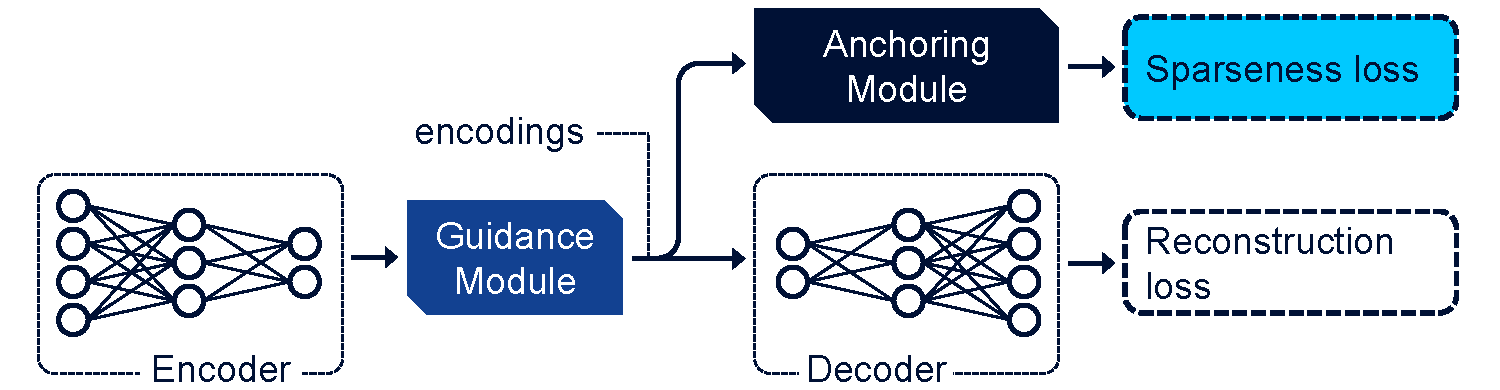
\includegraphics[width=\linewidth]{figures/06_sparse_clust/sca_overview/sca_overview.pdf}
				\caption[SCA modules]{The modules in the sparse clustering autoencoder.}
				\label{fig:sca_overview}
			\end{figure}
			
			Two autoencoder types are used in this work: a convolutional autoencoder, which contains convolutional and fully-connected layers, and a deep \ac{MLP}, which contains only fully-connected layers.
			The topologies of these will be discussed in more detail in later sections.
			The proposed clustering modules work with any common layer type.
			
			In the following, an encoded representation of an observation is referred to as an encoded vector $Q = \{q_1, q_2, \dots, q_D\}$, or simply as an \emphnox{encoding}.
			An encoding is made up of individual numerical values $q_i,\: i \in [1, D]$, also called \emphnox{activations}.
			Both the original observations and the encodings are vectors, which can also be thought of as single points in many-dimensional spaces.
			This is important, as most of the discussion is approached from a geometrical perspective.
			
		\subsection{From Sparseness to Convex Combinations}
		
			Generally, activation sparseness in a neural net means that in any activation vector (propagated tensor), only a limited number of activations take non-zero values.
			Sparseness can be desirable for regularization, or for lowering memory consumption and speeding up processing with the use of sparse matrix encoding and calculations.
			Usually, sparseness is enforced by masking, i.e.: non-desired activations are multiplied by $0$, ``turning off'' the activation and any backpropagation of gradients through the neuron.
			Deciding which activations to mask is net- and use-case-specific.
			
			One such specific use of activation sparseness is described in $k$-Sparse Autoencoders \cite{ksparse}.
			In the paper, the authors show that by only allowing the $k$ largest activations in each encoding to propagate further ($k$-sparseness), the autoencoder assigns expansive features (i.e. encompassing many aspects, a larger part of an observation) to individual activations.
			This effect is increased as $k$ is decreased.
			Naturally, we concluded that by only allowing the single largest activation to propagate ($1$-sparseness), each activation would represent most expansive feature possible, i.e. an entire observation.
			While early experimentation has shown that this is true, unfortunately this does not result in a clustering (logical grouping of observations), as allowing for a single activation to propagate still leaves a wide range of possible values for that activation, each of which can represent wildly different observations.
			
			Preferably, to achieve clustering, we would like to collect encodings around certain points in the encoded space, which, in the case of $1$-sparseness, means that we want to fix which value the single active neuron can take.
			The simplest choice for that value is $1$, which means that any observation is encoded into a $1$-hot vector, i.e: a vector that is filled with $0$s, except for a single position that contains a $1$.
			This can be seen as clustering or quantization, where the position of the $1$ activation defines which group the observation is assigned to.
			The number of possible clusters in this case is limited by the number of neurons in the middle layer of the autoencoder, i.e: the dimensionality of the encoding space, $D$.
			
			Spareness has to be gradually introduced during training, in order not to excessively disturb the formed encoding structure, to give time for the net to align to the new sparseness criteria \cite{ksparse}.
			This means that there needs to be a continuous transition defined from no sparseness ($D$-sparseness) to $1$-sparseness, which needs to also translate into a continuous translation from no clustering to full clustering.
			For this reason, net is enforced to represent encodings as \emphix{convex combinations}{convex combination} of the clusters, reminiscent of class probabilities.
			Mechanically, this baseline criteria means that:
			\begin{itemize}
				\item Activations are limited to the range of $[0, 1]$
				\item Activations in an encoding vector sum to $1$
			\end{itemize}
		
			\begin{figure}[ht]
				\centering
				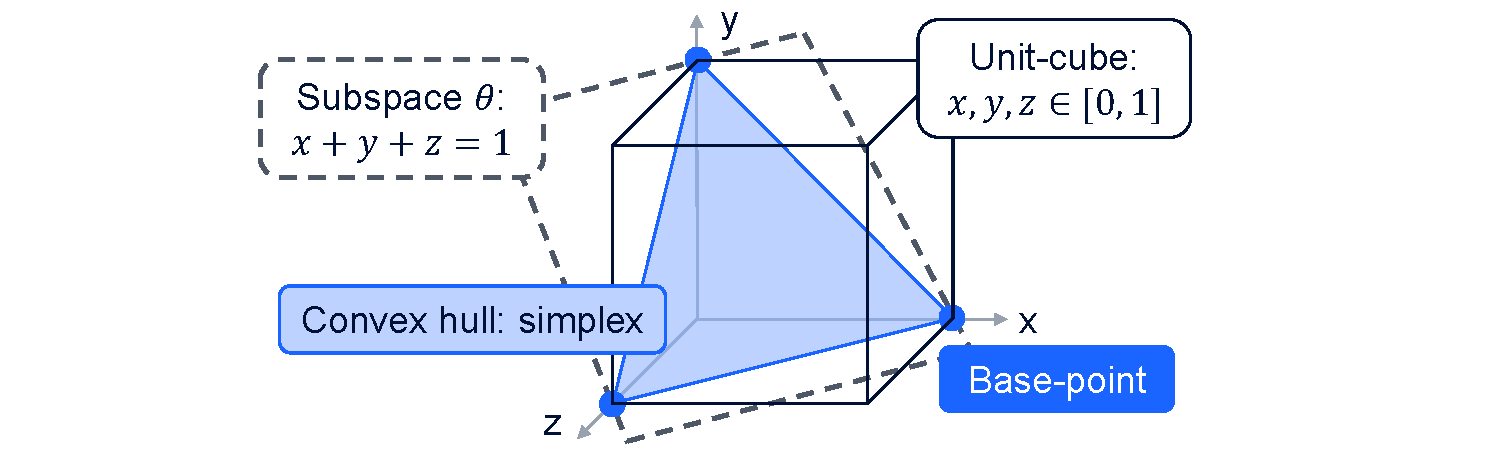
\includegraphics[width=\linewidth]{figures/06_sparse_clust/simplex/simplex.pdf}
				\caption[The simplex of convex combinations]{The simplex of convex combinations.}
				\label{fig:simplex}
			\end{figure}
			
			On top of these baseline criteria, we define the value $s$, representing sparseness.
			Let $C_{nz}(Q)$ be the number of elements of vector $Q$ that are non zero.
			Then, $s$ is defined as follows:
			\begin{equation*}
				s = C_{nz}(Q) - 1
			\end{equation*}
			
			The reason why we represent sparseness differently to conventional formulation is the following: the transition from no sparseness to full sparseness can be seen as a gradual limitation of the dimensionality of the space the encodings can use.
			Our definition of the sparseness value $s$ is equal to this dimensionality.
			The baseline criteria of convex combinations already means that the encoded points are confined to a regular \emphix{simplex}{simplex} (Fig.~\ref{fig:simplex}), the vertices of which are at the unit vectors along each dimension.
			We will refer to the unit vector positions as \emphix{base points}{base point} in the future.
			The simplex in a $D$-dimensional space is a convex hull in a $D-1$-dimensional affine subspace $\Theta$.
			
			The baseline restriction is also represented in $s$, since points within the simplex already adhere to the sparseness $s = D-1$.
			Lower $s$ values limit activations to sub-hulls of the simplex.
			As an example, in $4$ dimensions, the simplex is a $3$-dimensional regular tetrahedron, with an $s$-value of $3$.
			Lowering this $s$ to $2$, $1$, and then finally $0$, the activations are respectively restricted to the faces, edges, and vertices of the tetrahedron.
			The lowest sparseness value achievable is always $0$, at which point the encodings are forced into the base points (restricted to $1$-hot vectors), essentially realizing clustering/quantization.
			An illustration of this gradual limitation of freedom can be seen in Fig.~\ref{fig:limit_freedom}.
			All through the process, the activations retain their convex combination-like qualities.
			
			\begin{figure}[ht]
				\centering
				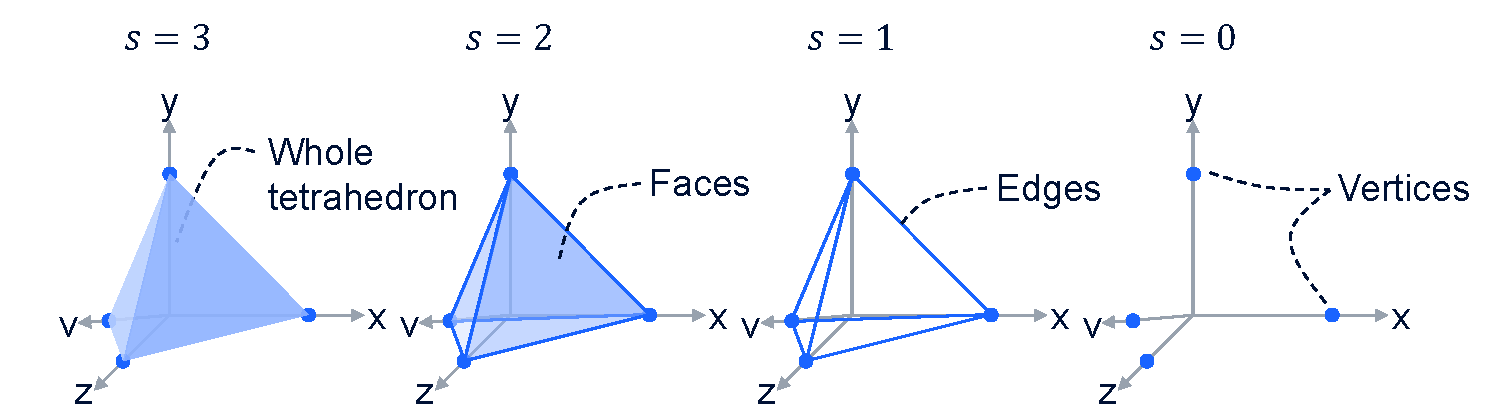
\includegraphics[width=\linewidth]{figures/06_sparse_clust/limit_freedom/limit_freedom.pdf}
				\caption[Gradual limitation of freedom in SCA]{Gradual limitation of freedom.}
				\label{fig:limit_freedom}
			\end{figure}
			
		\subsection{Anchoring Module - Sparseness Loss Calculation}
			
			As mentioned before, sparsity in neural nets is usually enforced by the masking of values, through multiplication by $0$.
			In many cases, this operation can mean a quite radical transformation of the activations, and as such it can easily degrade, or even destroy the learned encoding, as well as slow down training by suppressing gradient propagation in the net.
			In order to avoid this degradation, our method realizes a softer, more forgiving enforcement, by introducing a \emphnox{sparseness loss} on the embedding.
			The sparseness loss is calculated as a distance between the original encodings and their \emphnox{anchors}, the closest possible points to each encoding within the restricted space set by the value $s$.
			
			Generally, most neural nets are trained by backpropagation: a batch of observations is forward propagated, a single loss value is calculated on the results, which is then backpropagated to compute the gradients necessary to change the net weights.
			There are examples of neural nets, which are influenced by multiple losses (for example, using $L_1$ or $L_2$ regularization could constitute as such), but usually these affect the whole net, i.e. all layers of the net contribute to all losses.
			It is much rarer to have a loss only affecting a subset of weights.
			\ac{SCA} utilizes two losses: a reconstruction loss and a sparseness loss.
			The reconstruction loss is generic to autoencoders, usually a mean-squared-error loss, that affects the whole net.
			Contrary to this, the sparseness loss only affects the encoding part of the net and the guidance module.
			
			\begin{figure}[ht]
				\centering
				\subfloat[Sorting activations]{
					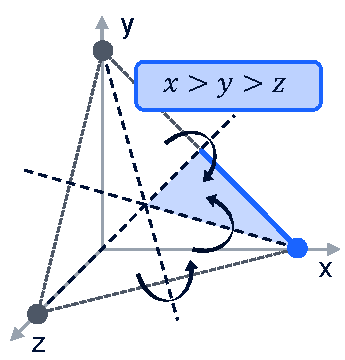
\includegraphics[width=0.24\linewidth]{figures/06_sparse_clust/core/core_rotate_mirror.pdf}
					\label{fig:core_rotate_mirror}
				}
				\subfloat[Generation of the new basis $\mathcal{A}$]{
					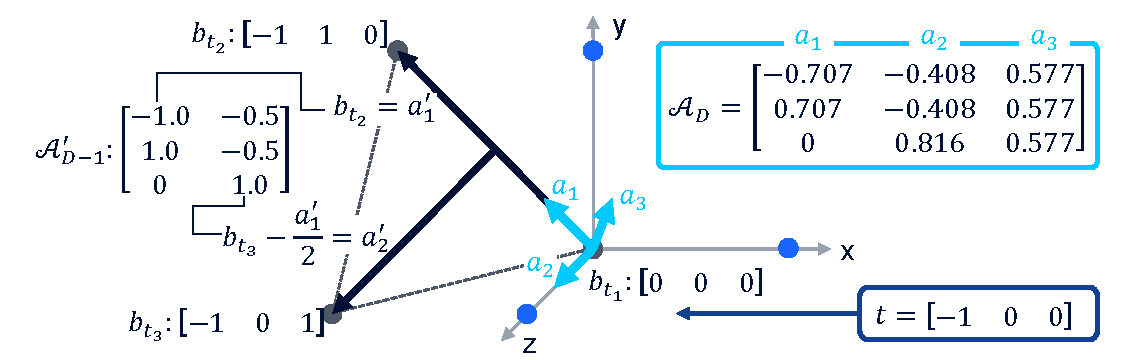
\includegraphics[width=0.75\linewidth]{figures/06_sparse_clust/core/core_rebase.pdf}
					\label{fig:core_rebase}
				}\\				
				\subfloat[Projection by masking]{
					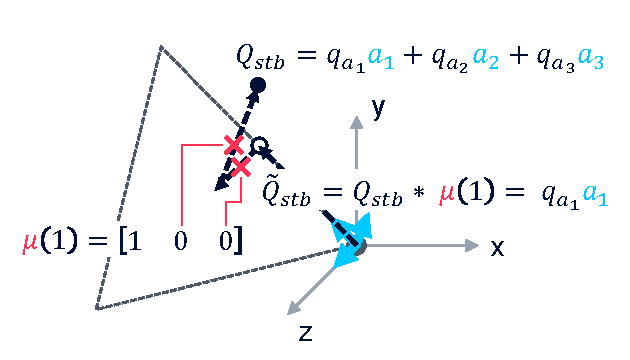
\includegraphics[width=0.42\linewidth]{figures/06_sparse_clust/core/core_project.pdf}
					\label{fig:core_project}
				}
				\caption[Anchor point generation in SCA]{The core steps in the generation of anchor point $\widetilde{Q}$.}
				\label{fig:core}
			\end{figure}
			
			Let us call the set of base-points, the non-negative points a unit distance from the origin on the axes $B = \{b_1, b_2, \dots, b_D\}$, where $b_i$ is a $1$-hot vector with the $1$-value in position $i$.
			For a given sparseness parameter $s \in [D-1, 0]$, the $D$ dimensional encoded representation $Q \in \mathbb{R}^D$ should lie on one of the the $s$-dimensional convex (sub-)hulls, which are defined by any of the subsets from $B$ with cardinality $s$.
			To create the sparsity loss acting on the encoded representation $Q$, an anchor point $\widetilde{Q}$ is calculated for every encoding, which is the projection of the encoding onto the closest sub-hull to $Q$.
			The projection is an orthogonal projection.
			The anchor describes the position where the encoded point should be according to the current sparseness level.
			The sparseness loss is then calculated as:
			\begin{equation}
				l_{sparse} = dist(Q, \widetilde{Q}),
			\end{equation}
			\noindent where $dist$ is the Euclidean or $L_2$ distance.
			
			Unfortunately, calculating the projection is a non-trivial task, because for $s < D$ there are multiple sub-hulls of the simplex, from which the closest one for each encoding needs to be found.
			In theory, this means that $\binom{D}{s}$ number of projections need to be computed, which is computationally intractable (for example, for $D = 16$ clusters with a sparseness of $s = 4$ means $1820$ different projections).
			In order to escape this complexity, the activations are sorted in a descending order, and the following operations work in this sorted space.
			From a geometric view, sorting rotates and mirrors all parts of the simplex into a single section (illustrated in Fig.~\ref{fig:core_rotate_mirror}), where only a single projection suffices to virtually implement all the the projections needed for an $s$ value.
			
			By using a translation of $-b_1$, the previously affine subspace $\Theta$ becomes a real subspace of $\mathbb{R}^D$ (the vector subspace associated to the affine subspace).
			Within this translated space, the task now is to calculate the anchor projection onto the $s$ dimensional subspace defined by the point set $\widetilde{B}_s = \{0, b_2 - b_1, \dots, b_s - b_1\}$.
			To effectively calculate anchors of encodings for every level of sparseness $s$, we change the basis of the encodings, by creating an new orthonormal basis $\mathcal{A}=\{a_1, a_2, \dots, a_D \}$, so that every subspace defined by the sub-basis $\mathcal{A}_s=\{a_1, a_2, \dots, a_s \}$ is parallel to the affine subspace $\Theta$.
			The calculation of the new basis can be simply done by using Gramm-Schmidt orgthogonalization on the points of $B$.
			This yields $\mathcal{A}_{D-1} = \{a_1, a_2, \dots, a_{D-1} \}$, with an additional base $a_D$ calculated as an orthonormal vector to $\mathcal{A}_{D-1}$, so that $\mathcal{A} = \mathcal{A}_D$ becomes a fully-ranked orthonormal basis (Fig.~\ref{fig:core_rebase}).
			To summarize the preparatory phase:
			\begin{enumerate}
				\item
					Let $B = \{b_1, b_2, \dots, b_D\}$, where $b_i$ is a $1$-hot vector with the $1$-value in position $i$.
					Translate $B$ by $-b_1$ and drop the first dimension, so $\widetilde{B} = \{b_2 - b_1, b_3 - b_1, \dots, b_D - b_1\}$.
					
				\item
					Orthogonalize $\widetilde{B}$ using the Gramm-Schmidt method, resulting in $\mathcal{A}_{D-1}$.
					
				\item
					Append the vector $a_D = \{\frac{1}{\sqrt{D}}, \frac{1}{\sqrt{D}}, \dots, \frac{1}{\sqrt{D}}\}$ to $\mathcal{A}_{D-1}$, which is unit length and orthogonal to all elements of $\mathcal{A}_{D-1}$, resulting in $\mathcal{A} = \mathcal{A}_D$.
					This makes $\mathcal{A}$ an orthonormal base of $\mathbb{R}^D$. This is our new base.
					
				\item
					Store $\mathcal{A}$ and $t$ as the new base change parameters.
			\end{enumerate}
			
			The sorting and translation has to be done on the encodings which are to be projected.
			After the translation, the base change is applied to $\mathcal{A}$.
			In this modified basis the projection to the $s$-sparse subspace can be done by masking the last $D-s$ bases.
			This is done similar to regular sparseness enforcement, by multiplying the activations with the mask $\mu(s) = (1,\dots,1,1,0,\dots,0)$, in which the first $s$ elements are $1$, and the rest $0$ (Fig.~\ref{fig:core_project}).
			Since the base change needs to be precomputed only once before training, this procedure enables us to efficiently project for different $s$ values, without the need for lengthy recomputations.
			So far, the sparseness computation is as follows:
			
%			\setcounter{equation}{0}
%			\begin{align}
%				\text{Sort activations:}\quad						Q_s &= sort(Q)											\\
%				\text{Translate:}\quad 								Q_{st} &= Q_s - t										\\
%				\text{Change to the new basis:}\quad 				Q_{stb} &= Q_{st}\mathcal{A}^T							\\
%				\text{Project by masking:}\quad 					\widetilde{Q}_{stb} &= Q_{stb} * \mu(s)					\\
%				\text{Re-base to original base:}\quad 				\widetilde{Q}_{st} &= \widetilde{Q}_{stb}\mathcal{A}	\\
%				\text{Re-translate:}\quad 							\widetilde{Q}_{s} &= \widetilde{Q}_{st} + t				\\
%				\text{Unsort activations:}\quad 					\widetilde{Q} &= unsort(\widetilde{Q}_{s})				\\
%				\text{Compute loss:}\quad 							l_{sparse} &= dist(Q, \widetilde{Q})
%			\end{align}
			
			\begin{algorithm}[!ht]
				\SetAlgoLined
				\newcommand{\nosemic}{\SetEndCharOfAlgoLine{\relax}}   % Drop semi-colon
				\newcommand{\dosemic}{\SetEndCharOfAlgoLine{\string;}} % Reinstate semi-colon
				\newcommand{\pushline}{\Indp}                          % Indent
				\newcommand{\popline}{\Indm\dosemic}                   % Undent		
				\let\oldnl\nl                                          % Store \nl in \oldnl
				\newcommand{\nonl}{\renewcommand{\nl}{\let\nl\oldnl}}  % Remove line number for one line
				
				\SetKwInput{Kw}{Required}
				\Kw{Orthonormal basis $\mathcal{A}$ and translation vector $t$}
				\Kw{Masking vector $\mu(s)$ set by sparseness value $s$}
				\Kw{Activation vector $Q$}
				
				\nosemic\nonl \;
				
				\dosemic Sort activations: $Q_s = sort(Q)$\;
				Translate: $Q_{st} = Q_s - t$\;
				Change to the new basis: $Q_{stb} = Q_{st}\mathcal{A}^T$\;
				Project by masking: $\widetilde{Q}_{stb} = Q_{stb} * \mu(s)$\;
				Rebase to original base: $\widetilde{Q}_{st} = \widetilde{Q}_{stb}\mathcal{A}$\;
				Retranslate: $\widetilde{Q}_{s} = \widetilde{Q}_{st} + t$\;
				Unsort activations: $\widetilde{Q} = unsort(\widetilde{Q}_{s})$\;
				Compute loss: $l_{sparse} = dist(Q, \widetilde{Q})$\;
				
				\caption[Long-form sparseness loss in SCA]{The long form of the sparseness loss calculation}
				\label{alg:sparse_loss_long}
			\end{algorithm}
			
			Fortunately, if the user has no need of the actual anchor points (for visualization, or debugging), steps $5$-$7$ can be omitted, almost halving the required computations.
			This is because, although a general basis change can be non-distance-preserving, the change between two orthonormal bases is an isometry, and as such preserves distances.
			This is also true for translation.
			Coordinate sorting would not be distance preserving between encodings, but it is distance preserving between every encoding and its corresponding anchor.
			This means that the distance between the original encoding and its projection remains the same through the whole process.
			This allows us to calculate the loss immediately after step $5$ as a function of $Q_{stb}$ and $\widetilde{Q}_{stb}$.
			Additionally, for further speedup, the masking operation can be done to the basis $\mathcal{A}$ itself instead of the encodings, which avoids a significant amount of computation.
			The shortened procedure is shown on Alg.~\ref{alg:sparse_loss_short}.
			
%			\setcounter{equation}{0}
%			\begin{align}
%				\text{Sort activations:}\quad						Q_s &= sort(Q)											\\
%				\text{Translate:}\quad 								Q_{st} &= Q_s - t										\\
%				\text{Mask basis:}\quad 							\widetilde{\mathcal{A}} &= \mathcal{A} * \mu(s)			\\
%				\text{Change to the new basis:}\quad 				\widetilde{Q}_{stb} &= Q_{st}\widetilde{\mathcal{A}}^T	\\					
%				\text{Compute loss:}\quad 							l_{sparse} &= dist(Q_{stb}, \widetilde{Q}_{stb})
%			\end{align}
			
			\begin{algorithm}[!ht]
				\SetAlgoLined
				\newcommand{\nosemic}{\SetEndCharOfAlgoLine{\relax}}   % Drop semi-colon
				\newcommand{\dosemic}{\SetEndCharOfAlgoLine{\string;}} % Reinstate semi-colon
				\newcommand{\pushline}{\Indp}                          % Indent
				\newcommand{\popline}{\Indm\dosemic}                   % Undent		
				\let\oldnl\nl                                          % Store \nl in \oldnl
				\newcommand{\nonl}{\renewcommand{\nl}{\let\nl\oldnl}}  % Remove line number for one line
				
				\SetKwInput{Kw}{Required}
				\Kw{Orthonormal basis $\mathcal{A}$ and translation vector $t$}
				\Kw{Masking vector $\mu(s)$ set by sparseness value $s$}
				\Kw{Activation vector $Q$}
				
				\nosemic\nonl \;
				
				\dosemic Sort activations: $Q_s = sort(Q)$\;
				Translate: $Q_{st} = Q_s - t$\;
				Mask basis: $\widetilde{\mathcal{A}} = \mathcal{A} * \mu(s)$\;
				Change to the new basis: $\widetilde{Q}_{stb} = Q_{st}\widetilde{\mathcal{A}}^T$\;					
				Compute loss: $l_{sparse} = dist(Q_{stb}, \widetilde{Q}_{stb})$\;
				
				\caption[Short-form sparseness loss in SCA]{The shortened form of the sparseness loss calculation}
				\label{alg:sparse_loss_short}
			\end{algorithm}
			
		\subsection{Guidance Module}
			
			The anchoring module provides the sparseness loss, but does not directly interact with the encodings.
			Contrarily, the guidance module, which is located in the middle of the autoencoder and precedes the anchoring module, does directly change the activations.
			One of the tasks of this module is to limit the encoding activations to the range of $[0, 1]$, by using a sigmoid nonlinearity, fulfilling one of the baseline requirements for convex combinations.
			The sigmoid nonlinearity ensures that the encodings fall within the unit hypercube in $\mathbb{R}^D$, turning the linear projection onto the affine subspace $\Theta$ into a projection onto the simplex.
			
			Many clustering algorithms have explicit mechanisms, often an additional loss, that tries to even out cluster populations.
			Without any additional mechanisms, our method runs into the problem of not properly exploring the encoding space at the beginning of the training.
			This leads to a reduced performance due to the encoding not utilizing all the available clusters for representation.
			Instead of an additional loss, we use a weight-shared batch-normalization layer before the sigmoid nonlinearity.
			Internally this layer centers the activations around $0$, by implementing:
			
			\begin{equation}
				\label{eq:guidance}
				y_{bn} = \frac{x - \mathrm{mean}(x)}{\mathrm{std}(x)}*p_{scale} + p_{offset}.	
			\end{equation}
			
			In Eq.~\ref{eq:guidance}, $x$ denotes the input, while $p_{scale}$ and $p_{offset}$ are learnable parameters of the batch normalization layer.
			The original idea behind batch-normalization is that at the start of the training, the normalization centers the activations, while the learnable parameters are initialized as neutral values, $p_{scale} = 1$ and $p_{offset} = 0$, not affecting the activations.
			The centering helps in the early training by easing discovery of the activation space, while later in the training, the net is able to counteract possibly unwanted normalization by separately changing the learnable parameters for any feature.
			In our case, to aid the even distribution of encodings all through the training, the learnable parameters are shared across features.
			This retains the centering effect of the batch normalization layer, but gives the net enough flexibility to adhere to the required sparseness.
			
		\subsection{Training}
			
			Weight decay, or $L_2$ regularization is a common technique to reduce the propensity of overfitting in neural nets.
			Originally formulated as an additional loss, the common simple weight decay implementation works by decaying weights by a small amount before every update.
			The regularization effect can be very important in the case of \acp{SCA}, in order to achieve a sensible clustering.
			Weight decay constrains the complexity of the encoding and decoding functions, so that small changes in the original data-space cannot result in arbitrarily large changes in the encoding space.
			The effect is that the net is forced to place similar observations in close proximity in the encoding space, which results in homogeneous, meaningful clusters.
			
			Generally, weight decay is used on all weights of the net, except the shared $p_{scale} = 1$ and $p_{offset}$ parameters in the guidance module.
			After a warm-up period, the power of the weight decay is gradually increased during training.
			The sparseness value $s$ is similarly handled, decreasing its value from $D-1$ to the goal (which is usually between $0$ and $1$), to ease the transition from a regular representation to a clustering.
			Figure~\ref{fig:sca_training} shows a typical training, highlighting the different phases and how the reconstruction loss and the sparseness loss develops, as well as how the weight decay and sparseness parameters are set.
			
			\begin{figure}[ht]
				\centering
				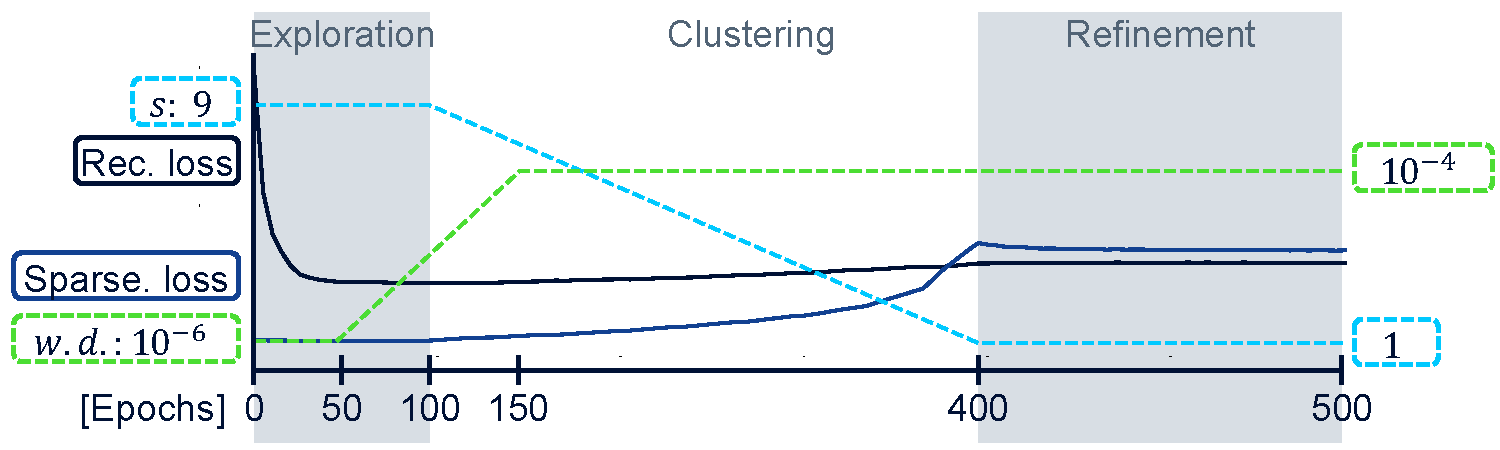
\includegraphics[width=0.8\linewidth]{figures/06_sparse_clust/sca_training/sca_training.pdf}
				\caption[Parameters and phases during a typical SCA training]{Parameters and phases during a typical SCA training.}
				\label{fig:sca_training}
			\end{figure}
			
			In the \emphnox{exploration phase} the sparseness parameter is held at the initial $D-1$ value, which only limits the activations onto the simplex.
			This leaves a large amount of freedom for the autoencoder to explore the encoding space and establish a mapping that can later be focused onto the simplex.
			In the \emphnox{clustering phase}, the $s$ parameter is gradually decreased to encourage the grouping of encodings.
			The \emphnox{refinement phase} then allows the net to smooth out imperfections that might have arisen during the clustering phase.
			
			During the development of \ac{SCA}, we often used scatter-plots of the encoded activations, to make sure the net behaves correctly.
			We found the best way to plot encodings is to project them into a $2$-dimensional space so that the base points are arranged on a circle, going around clockwise.
			Of course, the projection can be misleading, as one has to keep in mind that all base points are equidistant from each other in the encoding space, however, the plots give a good impression of how the encoding develops as sparseness is increased.
			Some of these plots can be seen in Fig.~\ref{fig:sca_training_scatter}, taken from different epochs during the training depicted in Fig.~\ref{fig:sca_training}.
			
			\begin{figure}[ht]
				\centering
				\subfloat[Epoch 50]{
					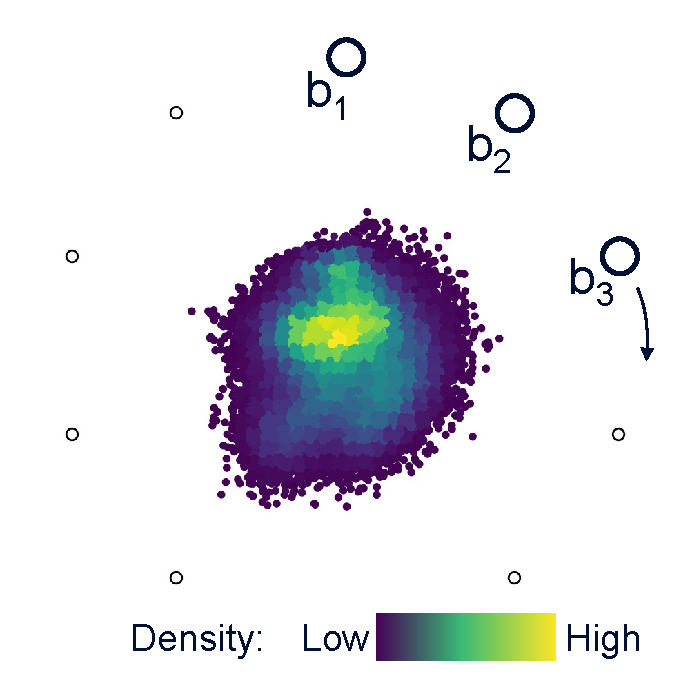
\includegraphics[width=0.48\linewidth]{figures/06_sparse_clust/sca_training_scatter/scatter_050.pdf}
				}
				\subfloat[Epoch 200]{
					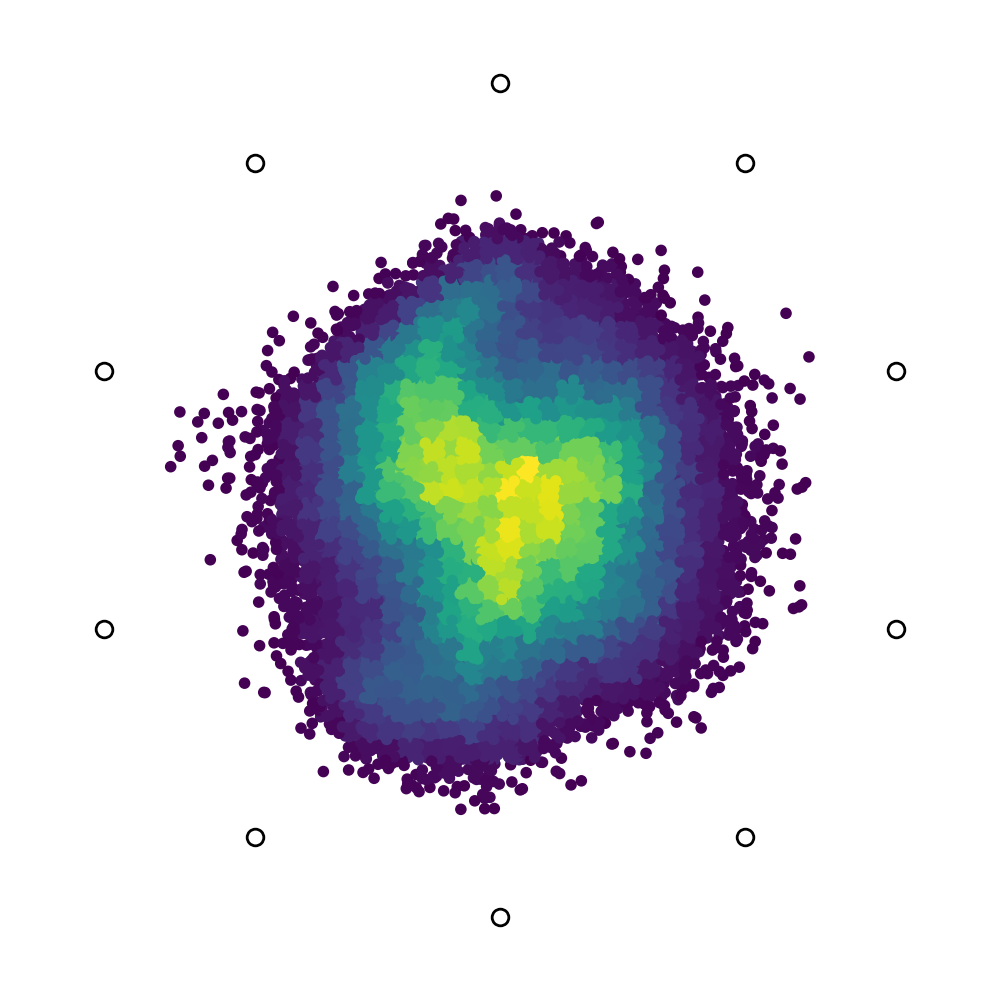
\includegraphics[width=0.48\linewidth]{figures/06_sparse_clust/sca_training_scatter/mnist_training_200.png}
				}\\				
				\subfloat[Epoch 350]{
					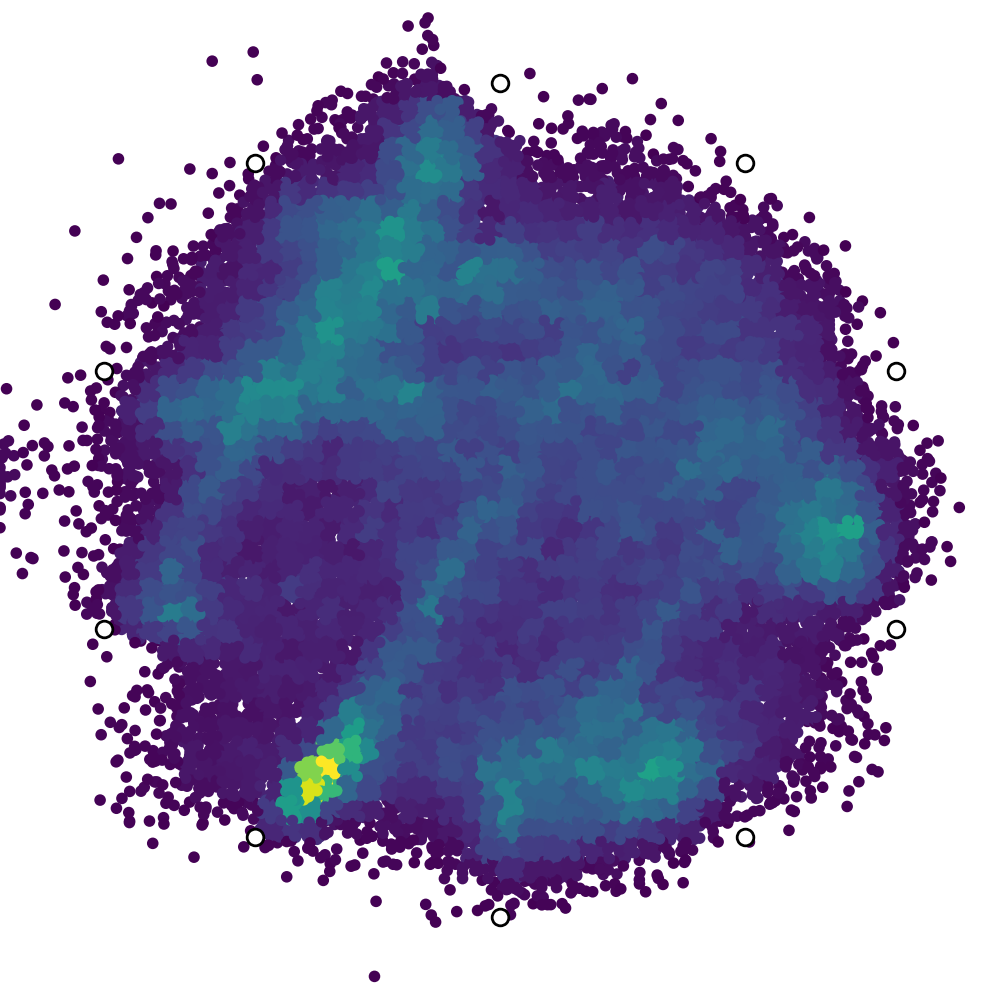
\includegraphics[width=0.48\linewidth]{figures/06_sparse_clust/sca_training_scatter/mnist_training_350.png}
				}
				\subfloat[Epoch 500]{
					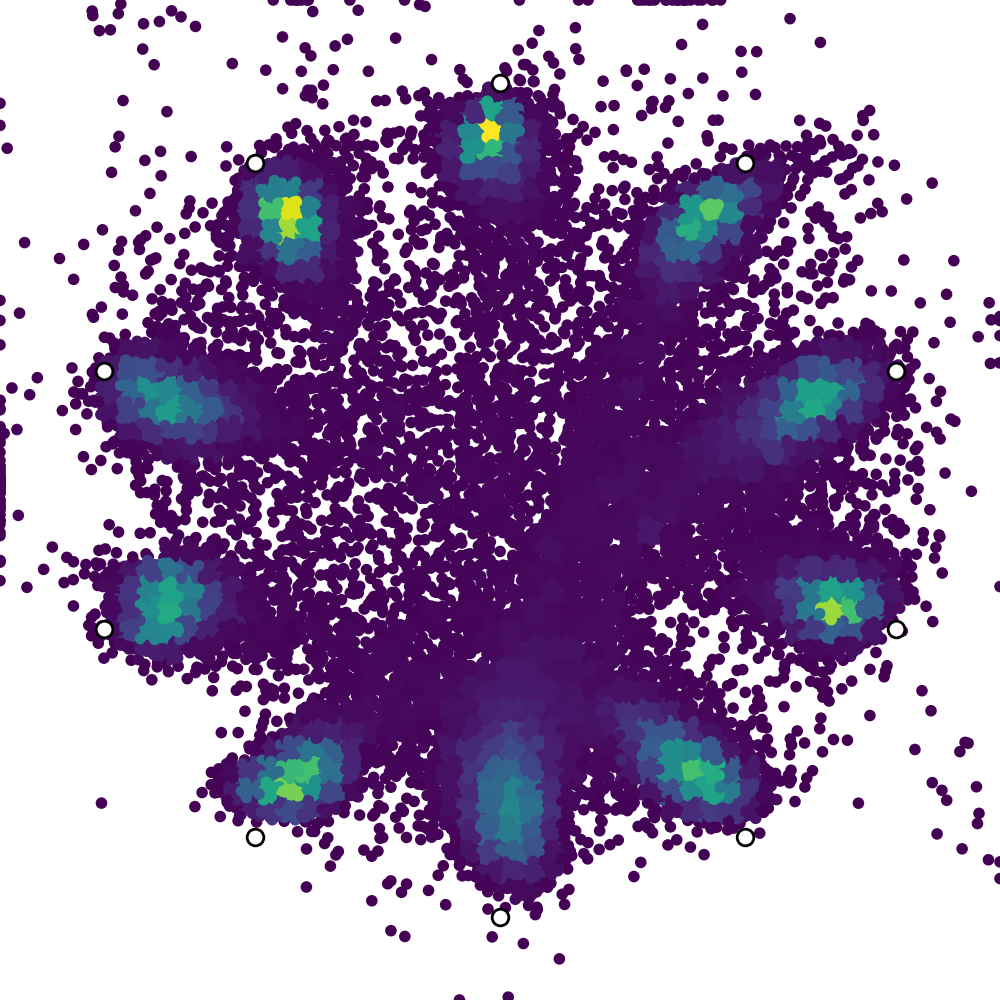
\includegraphics[width=0.48\linewidth]{figures/06_sparse_clust/sca_training_scatter/mnist_training_500.png}
				}
				\caption[Projected scatter plots of the encodings during SCA training]{Projected scatter plots of the encodings during SCA training.}
				\label{fig:sca_training_scatter}
			\end{figure}
			
		\subsection{Related Work in Mobile Network Automation}
			
			Clustering can be a useful tool for network management use cases where autonomous agency is required, because the conditions with which the system will be working are unknown at the design time.
			One group of such use cases fall under the Self-healing aspect of \ac{SON} \cite{SONbook}.
			Self-healing is envisioned as one of the final stages towards complete autonomy, where \acp{SON} are be able to detect, diagnose, and recover from previously known and even unknown failures in the network.
			The first step of this process is the detection of anomalous behavior:
			
			\begin{itemize}
				\item
					Static anomalous cell behavior can be caused by erroneous \ac{CM} settings, especially so when the settings are autonomously changed by multiple \ac{SON} functions.
					In \cite{ciocarlie2014anomaly}, the \ac{HDP} clustering is used to detect \ac{CM} changes that cause a degradation, and to possibly roll back these changes.
				
				\item
					Dynamic anomalies in cell behavior can be caused by strange user behavior, software bugs, or hardware failure.
					In \cite{gajic2015improved}, such anomalies are detected with the help of the \ac{MGNG} clustering algorithm.
					A later improvement to this clustering method, called \ac{FRGNG} is proposed in \cite{gajic2015frgng}.
				
				\item
					A specific use case for anomaly detection in mobile networks is detection of sleeping cells.
					In \cite{chernogorov2011detection}, the \kmeans{} algorithm is used in an encoded space formed by diffusion maps on simulated radio measurements, in order to detect degraded or sleeping cells.				
			\end{itemize}
			
			While some of the clustering methods above are very complex, none of them are deep learning-based.
			The mentioned use cases rely on precise models for sensing specific network states.
			Simple models generated by statistical methods are prone to underfitting.
			Deep-learning-based clustering could be a better fit for these systems, by allowing for a modeling that focuses on deeper underlying logic in the data, and is in turn not prone to sensitivity issues.
						
		\subsection{Related Work and Comparison in Deep Clustering}
			
			Deep clustering algorithms utilize deep neural nets, such as deep \acp{AE} (\ac{MLP} and \ac{CNN}), \acp{VAE}, \acp{DBN} or \acp{GAN}.
			The structure of some of these algorithms is similar to \ac{SCA}, where the goal of the net is to best reconstruct the original observations, but with an additional criteria present during training.
			As such, most of these net topologies are autoencoder-like, forcing a simplification and a reconstruction in the model.
			A good overview of the recent deep clustering algorithms can be found in \cite{aljalbout2018clustering}.
			
			What distinguishes \ac{SCA} from other deep clustering algorithms is the way clustering is achieved.
			In other algorithms -- such as  \ac{DEC} -- the encoded activations are not forced to be sparse representation, rather, cluster centroids are estimated by parameters or an additional statistical clustering algorithm, such as \kmeans{}.
			To influence a ``confident'' clustering in these algorithms, the additional clustering loss moves the activations to their closest centroids, while also possibly moving the centroids away from each other, in order to minimize within-cluster scattering, but maximize between-cluster distinction.
			
			The algorithms are evaluated on datasets where class associations are known.
			The clustering algorithms' task is to form clusters of observations that match the original classes closely (obviously, without the knowledge of these class associations).
			The most common datasets are images, as these contain strong underlying logic in the observations that are hard to extract with non-deep learning methods.
			The dataset of choice in many of the papers is the MNIST dataset, a collection of $60$ thousand handwritten digits scanned from US postal codes, stored as $28$-by-$28$ pixel grayscale images.
			In this case, the clustering algorithm's task is to automatically associate each image to one of $10$ clusters, each representing one of the digits.
			
			\begin{figure}[ht]
				\centering
				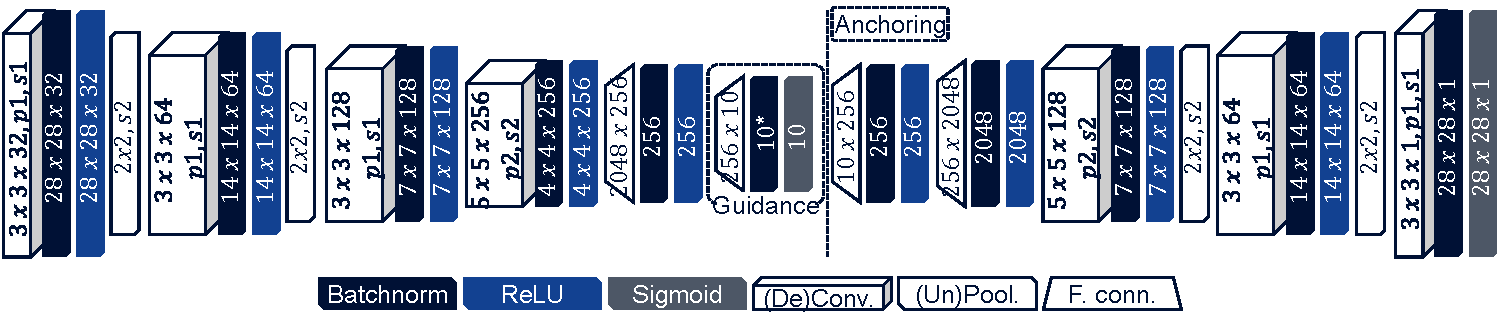
\includegraphics[width=\linewidth]{figures/06_sparse_clust/topology_conv/topology_conv.pdf}
				\caption[CNN AE topology used for MNIST in the SCA evaluation]{The convolutional autoencoder net topology used for deep clustering of the MNIST dataset.}
				\label{fig:topology_conv}
			\end{figure}
			
			Performance is measured against the original class associations, with metrics that are invariant to cluster association permutations.
			One such metric is \ac{NMI}, which takes the value $0$ in case of no correlation between cluster and class associations, and $1$ if there is a perfect match between the two.
			Following is a table from \cite{aljalbout2018clustering} (Tab.~\ref{tab:deepcluster}), that compares the performance of our algorithm with recent deep clustering algorithms, measured as the \ac{NMI} on the MNIST dataset.			
					
			\begin{table}[t]
				\centering
				\renewcommand*{\arraystretch}{1.2}
				\begin{tabular}{l l l|r}					
					Method										&Architecture	&Clustering alg.		&NMI		\\
					\hline
					\kmeans{}									&-				&-						&$0.481$	\\
					DEC	\cite{dec}								&\ac{MLP}		&Net est. params.		&$0.800$	\\
					DCN	\cite{dcn}								&\ac{MLP}		&Net est. params.		&$0.810$	\\
					\rowcolor{hlbluedark}SCA					&\ac{CNN}		&-						&$0.839$	\\
					UMMC \cite{umcc}							&\ac{DBN}		&\kmeans{}				&$0.864$	\\
					CCNN \cite{ccnn}							&\ac{CNN}		&\kmeans{}				&$0.876$	\\
					JULE \cite{jule}							&\ac{CNN}		&Agglomerative clust.	&$0.915$	\\
					DEPICT \cite{depict}						&\ac{CNN}		&Net est. params.		&$0.916$	\\
					DBC	\cite{dbc}								&\ac{CNN}		&\kmeans{}				&$0.917$	\\
					TAX	\cite{aljalbout2018clustering}			&\ac{CNN}		&Net est. params.		&$0.923$
				\end{tabular}
				\caption[Deep clustering algorithm performance comparison on MNIST]{Deep clustering algorithm performance comparison on MNIST.}
				\label{tab:deepcluster}
			\end{table}
			
			% ITT - :'(
			
			The performance of our algorithm is highlighted with blue.
			For reference, the performance of the regular \kmeans{} algorithm is also included, as a representative of traditional algorithms.
			To achieve this clustering task, here a deep autoencoding \ac{CNN} was used with sparseness loss injected at the middle of the net, as illustrated by the topology in Fig.~\ref{fig:topology_conv}.
			Although other algorithms did perform better, we see our method as competitive.
			At the time, we did not consider this performance to be the absolute best achievable, as there remain certain quirks, as well as a very irregular performance between trainings, which we hoped to eliminate in the future.
			The performance of the \ac{SCA} algorithm in clustering tasks will be discussed further in Sec.~\ref{cha:sparse_clust:sec:bias}.
			
		\subsection{Example Use of SCA: Cell Anomaly Detection }
			
			This section is meant as a demonstration of the ease of understanding gained by working with meaningful clusters on multi-dimensional network management data.
			The example given here shows how to explore network data using \ac{SCA} to get a general overview of the network, and look for anomalous/misconfigured cells.
			With the use of the state transition graph, $3$ types of anomalous behavior can be defined (Fig.~\ref{fig:stategraph_anomalies}):
			\begin{enumerate}
				\item
					\textbf{Anomalous states} are labeled states (already present in the training dataset) that are known to represent something abnormal.
					
				\item
					\textbf{Static anomalies} are measurements that fall outside of the populated parts in the model.
					
				\item
					\textbf{Dynamic anomalies} are (sequences of) state transitions that are not seen in normal operation.
			\end{enumerate}
			
			\begin{figure}[ht]
				\centering
				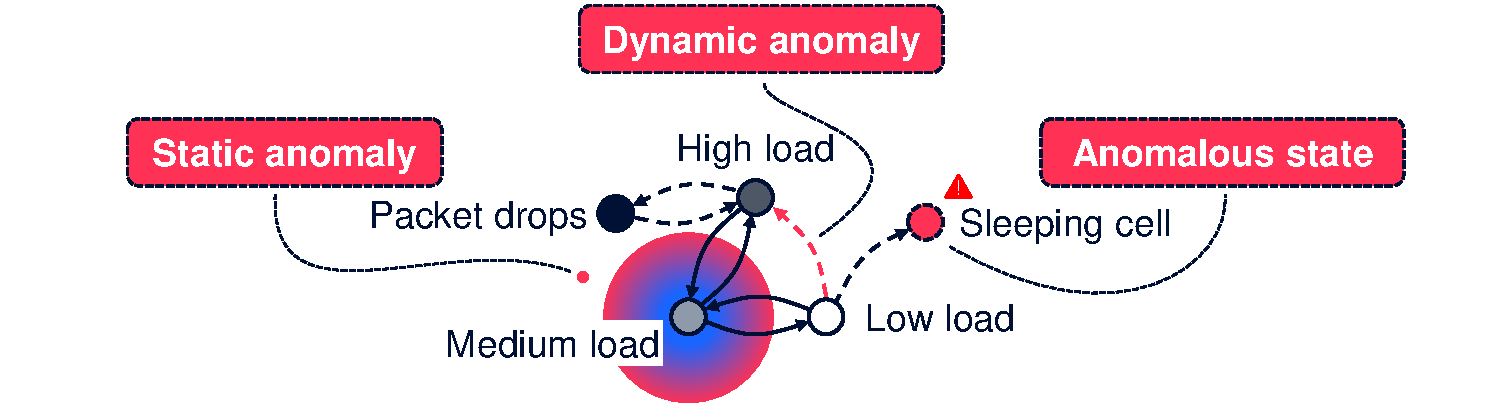
\includegraphics[width=\linewidth]{figures/06_sparse_clust/stategraph_anomalies/stategraph_anomalies.pdf}
				\caption[Anomalous behavior types in the network state transition graph]{Anomalous behavior types in the network state transition graph.}
				\label{fig:stategraph_anomalies}
			\end{figure}
			
			This evaluation focuses on anomalous states.
			To show an example of anomalous cell state detection, we have trained an \ac{SCA} on \ac{PM} data captured from a real mobile network.
			The dataset contains roughly $3$ months worth of hourly measurements from more than $2000$ cells, consisting of $17$ \acp{KPI}, which can be grouped into $5$ categories based on meaning, as shown on Tab.~\ref{tab:kpigroups}.
			
			\begin{table}[t]
				\centering
				\renewcommand*{\arraystretch}{1.2}
				\begin{tabular}{r|l}					
					\textbf{Users}					&Number of users, connection attempts/releases		\\
					\textbf{Volume / throughput}	&Data volume, PRB utilization, layer throughput		\\
					\textbf{Latency}				&Latency on radio									\\
					\textbf{Radio conditions}		&RSRP/Q, CQI										\\
					\textbf{Voice}					&Voice data volume, number of QCI 1 users
				\end{tabular}
				\caption[KPI groups collected for the SCA evaluation]{KPI groups collected.}
				\label{tab:kpigroups}
			\end{table}		
			
			The neural net used for this clustering was a deep \ac{MLP} autoencoder consisting of fully-connected layers, batch normalization layers and Leaky \ac{ReLU} nonlinearities \cite{maas2013rectifier}, the topology of which can be seen in Fig.~\ref{fig:topology_mlp}.
			The encoder and the decoder were mirrored equivalents, both consisting of $4$ layers.
			
			\begin{figure}[ht]
				\centering
				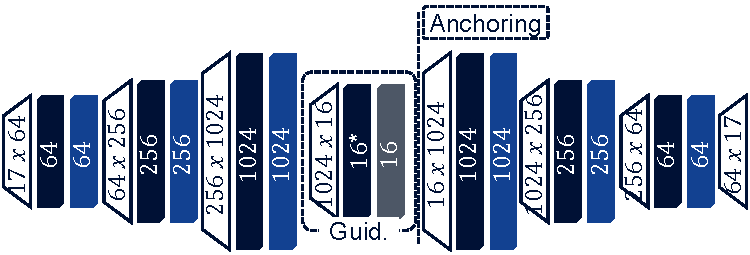
\includegraphics[width=0.5\linewidth]{figures/06_sparse_clust/topology_mlp/topology_mlp.pdf}
				\caption[MLP AE topology used for network data in the SCA evaluation]{The MLP autoencoder network topology used on network data.}
				\label{fig:topology_mlp}
			\end{figure}	
			
			We chose to use $16$ clusters for this demonstration, as too many would be hard to visualize.
			The choice is a little arbitrary, as in a typical scenario the user has no notion of how many real classes to expect in the data, a downside shared by many other clustering algorithms.
			Generally, the with more clusters used, cluster homogeneity increases, making the right choice for the number of clusters dependent on a tradeoff between homogeneity and complexity of the outcome.
			
			The sparsity parameter $s$ was continuously lowered from $15$ to $0.5$ during training, not $0.0$.
			This creates an encoding, that somewhat allows for binary combination of two network states, which helps in the identification of used transitions between the states. The final projection of the encoded activations can be seen in Fig.~\ref{fig:graph_scatter}, together with the corresponding network state graph.
			
			\begin{figure}[ht]
				\centering
				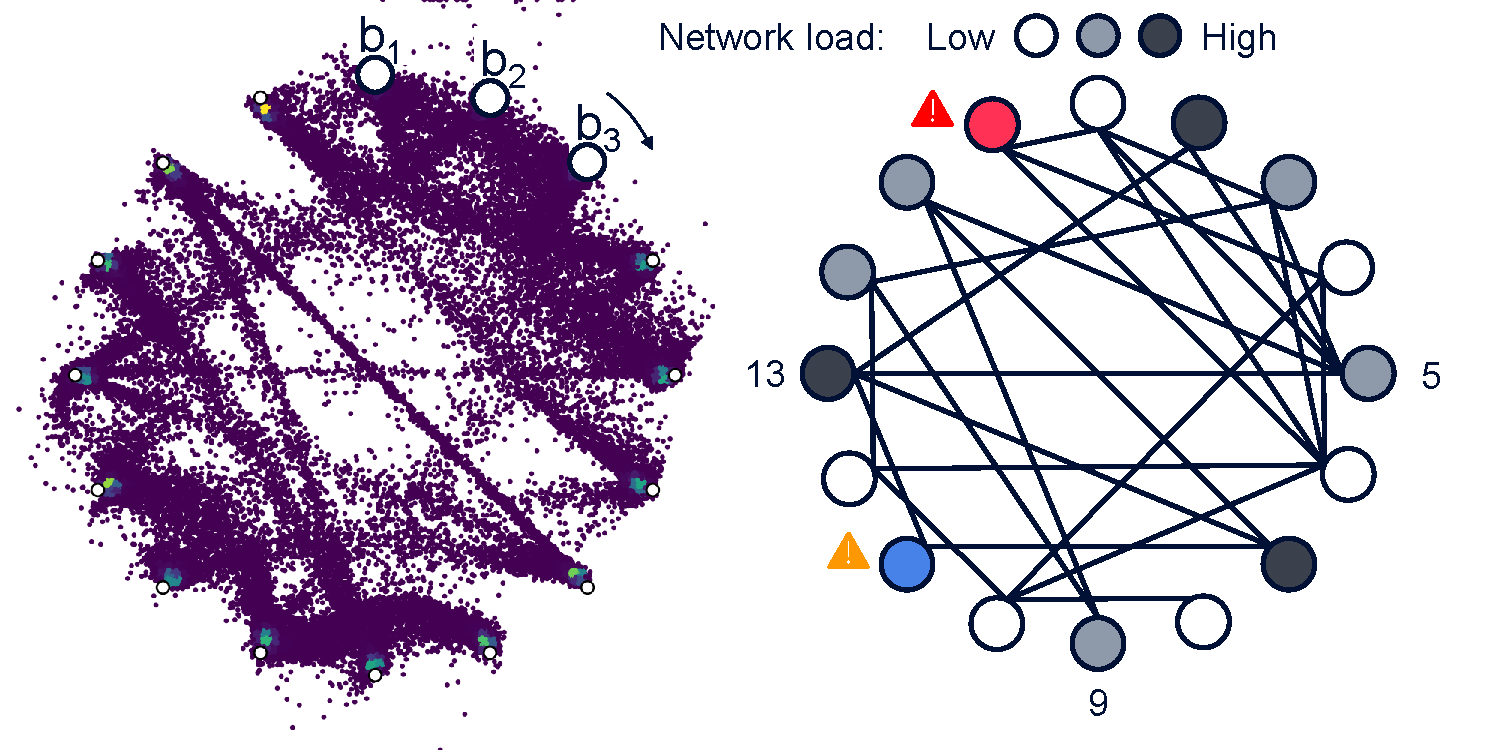
\includegraphics[width=\linewidth]{figures/06_sparse_clust/graph_scatter/graph_scatter.pdf}
				\caption[Network data as a state transition graph]{Network data encoded by SCA as activations (left), and the equivalent network state transition graph (right).}
				\label{fig:graph_scatter}
			\end{figure}
			
			Each observation was hard-assigned to the state with the largest activation in its encoding.
			The connections in the network state graph were established by looking at the network state transition sequences in the data: a connection is drawn between two states, if the number of transitions between the two clusters is above a certain threshold.
			There is a clear distinction in the number of transitions between often used and seldom used transitions, with often used transitions numbering in the $100$ thousands range, while seldom used ones only represented in the hundreds.
			We chose the cutoff threshold to be $1000$ transitions, with which the network state graph visually matches the scatter plot of the encoded activations.
			
			The prototypes (or centroids) of the states are obtained by decoding the $1$-hot encoding vectors in the encoding space back to the original \ac{KPI}-space.
			By looking at what these prototypes represent in the original \ac{KPI}-space (in the form of bar-charts), we were quickly able to deduce that most of the states correspond to different levels of network load, but represent mostly normal operation.
			In Fig.~\ref{fig:graph_scatter}, the states are colored from white to dark gray depending on the network load.
			However, states $11$ and $16$ stood out, showing strange behavior (highlighted as dark blue and red respectively).
			The \ac{KPI}-space prototypes of these states can be seen in Fig.~\ref{fig:bars_zoom}.
			All \acp{KPI} are shown as individually normalized features, with their mean being at $0$ and standard variation at $1$, thus, the vertical axis holds values in standard deviation.
			
			\begin{figure}[ht]
				\centering
				\subfloat[State $11$]{
					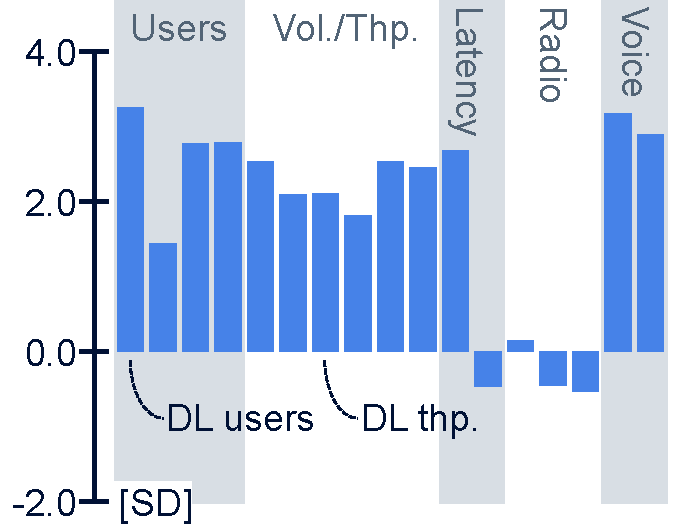
\includegraphics[width=0.46\linewidth]{figures/06_sparse_clust/bars_zoom/bars_11.pdf}
				}
				\subfloat[State $16$]{
					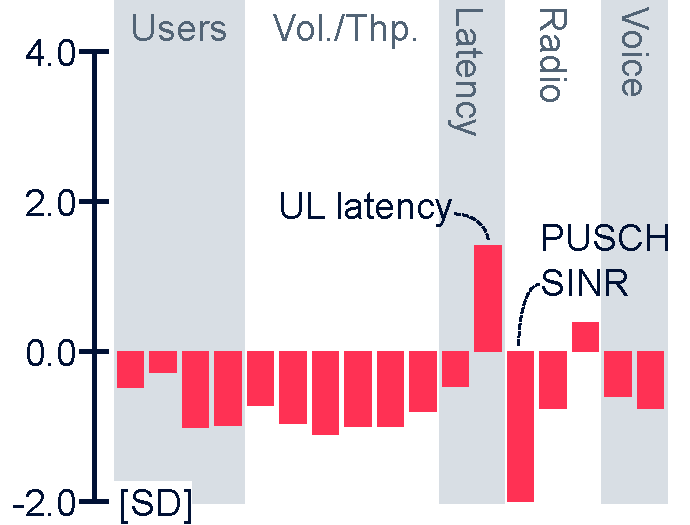
\includegraphics[width=0.46\linewidth]{figures/06_sparse_clust/bars_zoom/bars_16.pdf}
				}
				\caption[Anomalous network state prototypes]{Anomalous network state prototypes.}
				\label{fig:bars_zoom}
			\end{figure}
			
			State $11$ shows extremely high user numbers and throughput in the downlink, one which is not represented in any other state.
			State $16$, on the other hand, shows a situation with low cell load, but unreasonably high uplink latency, and abysmal uplink radio conditions.
			It is interesting to note, that state $11$ only has transitions from and to high load states, while state $16$ only low load states, which is also represented in Fig.~\ref{fig:bars_zoom}.
			Another important aspect to note is that out of all states, state $11$ and $16$ have the largest amount of self-transitions, meaning that these states were usually not temporary, rather, cells spent longer, continuous timeframes therein.
			
			\begin{figure}[ht]
				\centering
				\subfloat[State $11$]{
					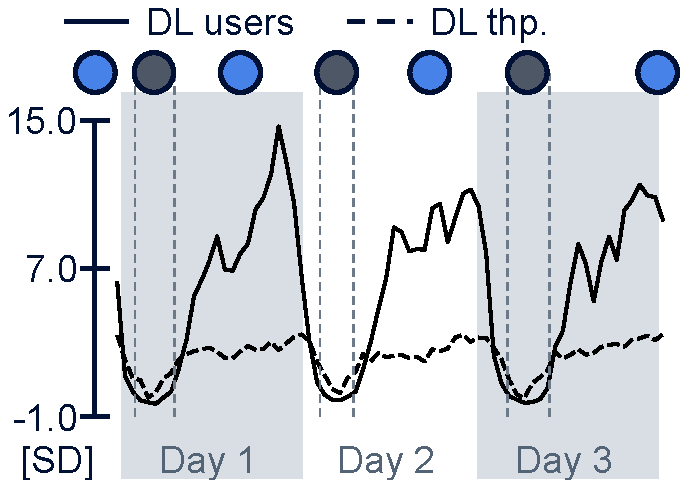
\includegraphics[width=0.48\linewidth]{figures/06_sparse_clust/lines_zoom/lines_11.pdf}
				}
				\subfloat[State $16$]{
					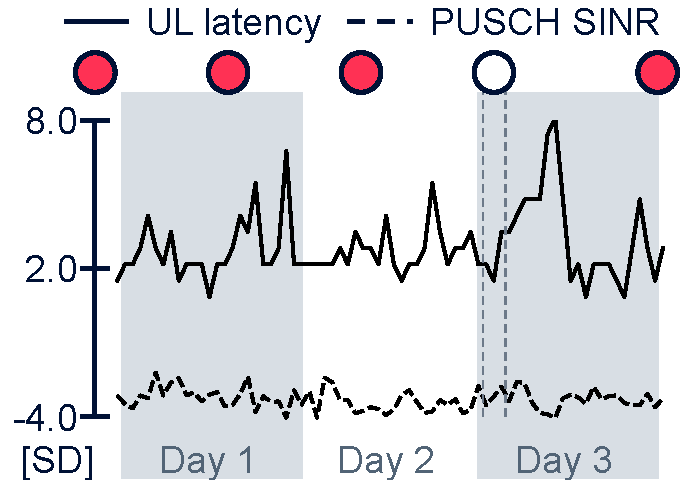
\includegraphics[width=0.48\linewidth]{figures/06_sparse_clust/lines_zoom/lines_16.pdf}
				}
				\caption[Anomalous network state sequences]{Anomalous network state sequences.}
				\label{fig:lines_zoom}
			\end{figure}
			
			Fig.~\ref{fig:lines_zoom} shows $3$ days of two cells with a high amount of time spent in state $11$ and $16$ respectively.
			Although a large portion of the time is spent therein, state $11$ turns out to be a somewhat temporary state, as cell $A1$ regularly leaves it.
			Contrarily, state $16$ seems to be more permanent, as cell $A2$ was continuously int that state for almost $2$ days.
			This can be verified also in Fig.~\ref{fig:maps}, where the cells are shown on the map and colored according to their state.
			During peak hours (3:00 PM), state $11$ is represented in many of the cells belonging to densely populated, urban areas, however, all cells leave this state in the off hours (3:00 AM).
			On the other hand, some cells in rural areas seem to be stuck in state $16$ for long periods of time.
			
			\begin{figure}[ht]
				\centering
				\subfloat[3:00 PM]{
					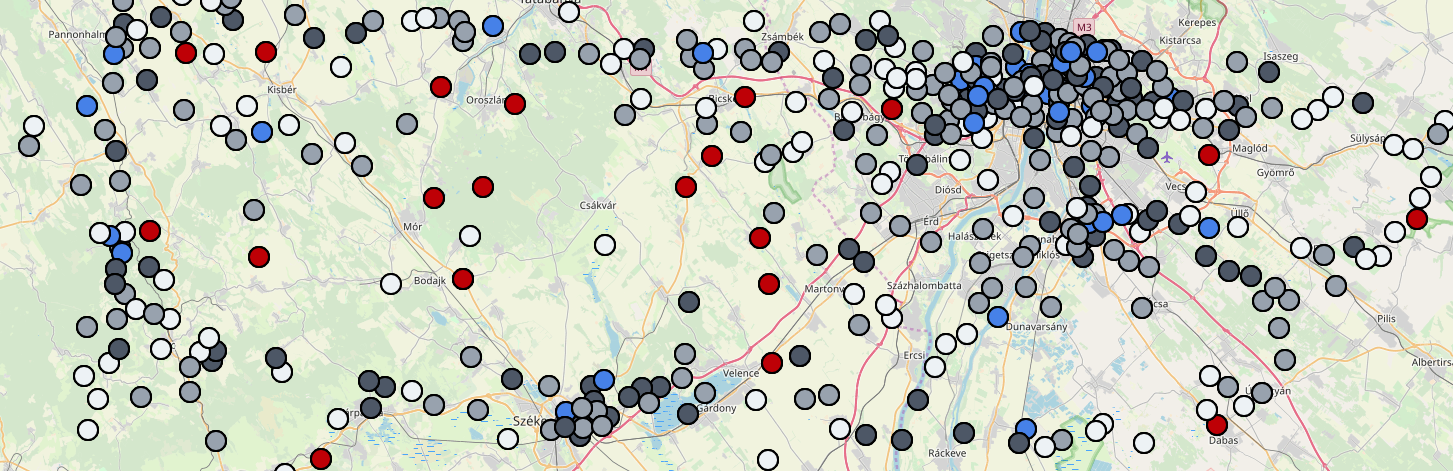
\includegraphics[width=0.98\linewidth]{figures/06_sparse_clust/maps/map_day_cut.png}
				}\\				
				\subfloat[3:00 AM]{
					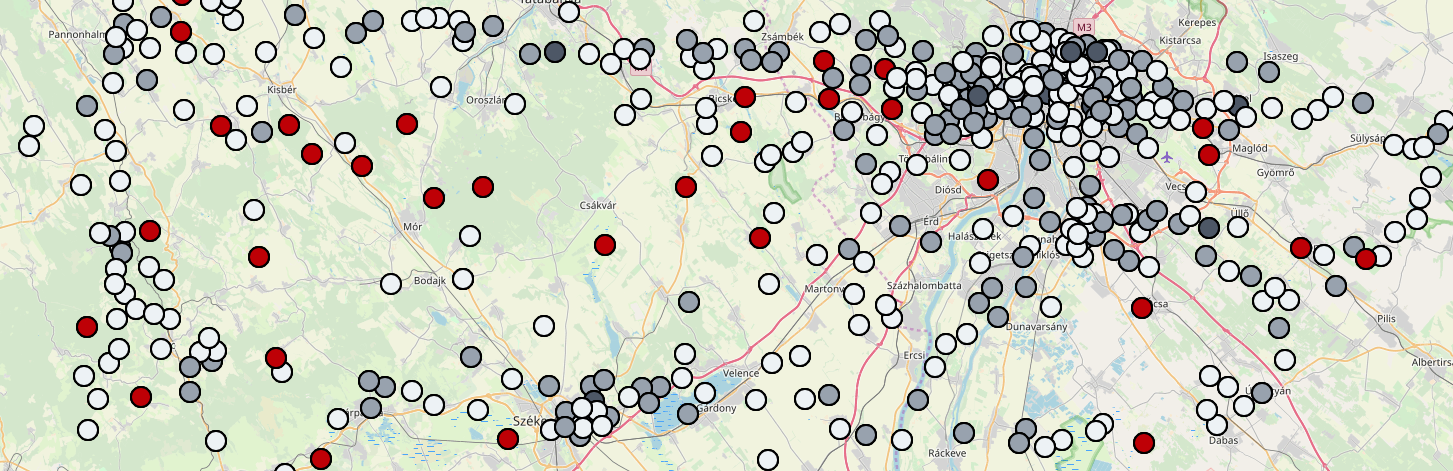
\includegraphics[width=0.98\linewidth]{figures/06_sparse_clust/maps/map_night_cut.png}
				}
				\caption[Maps of cell states at two different times in the day]{Maps of cell states at two different times in the day.}
				\label{fig:maps}
			\end{figure}
			
			Overall, we conclude that state $11$, although showing an extremely high load, does not represent a fault in itself.
			However, the cells that spend long, continuous timeframes in $16$, should be checked for possible misconfiguration, or a potential \ac{CCO} issue.
			
		\subsection{Conclusion and Critique}
		
			This chapter discussed a deep-neural-net-based clustering algorithm, that is meant to translate network data into a network state transition graph.
			A proposed implementation was explained from a geometrical perspective, and evaluated both quantitatively using a common dataset, and qualitatively using data from a real mobile network.			
			Moving forward, our goal was to improve the algorithm, and publish a paper including a thorough quantitative evaluation in common clustering scenarios with common datasets.
			However, this goal was ultimately never reached, as we realized there were fatal flaws in the algorithm, which impacted its performance in a clustering setting.
			These flaws -- the mistakes we made during design -- are not specific to \ac{SCA}, and we encountered them later in our research, pointing to a more general problem in \ac{DL} algorithm design.
			I think general a conclusion can be made using our \ac{SCA} design process as an example, thus the next section is dedicated to this discussion.
	
	\section{On Human Bias in DL Algorithms, Explainability}
		\label{cha:sparse_clust:sec:bias}
		
		\ac{SCA} is \ac{DNN}-based clustering algorithm, meant to be especially fit to translate network data into an easily understandable model, which we call a network state transition graph.
		While this intuitiveness was the main goal when developing the algorithm, we also wanted to realize some algorithmic aspects on a more mechanical level:
		\begin{enumerate}[label=\textbf{\alph*})]
			\item
				Many deep clustering methods use secondary, statistical clustering algorithms (such as \kmeans{}) to define clusters in their latent space, which introduce more parameters for the user to set, and in turn more possibilities where bias or misconfiguration can compromise the results.
				\ac{SCA} was designed to remove this additional clustering step, by forcing the autoencoder to move the clusters into predefined locations in the latent space.
				The idea behind this design decision was that, as the autoencoders usually have plenty of modeling power to encode into latent spaces even with constraints, there should be no need to add further complexity with a secondary clustering step.
				Thus, instead of a secondary clustering step defining the clusters, the (micro-)clusters in \ac{SCA} are immediately defined around predefined points in the latent space.
				At the time of this research, \ac{SCA}'s approach to deep clustering was not prevalent, and only recently have we encountered publications that undertake something similar, albeit through a quite different implementation.
			
			\item
				\ac{SCA} utilizes the latent observations -- mapped to predefined base-points -- as the only source of input to the decoder.
				We theorized that this way, the decoding has the greatest regularization effect on the latent space, and will not allow for misaligned mappings where multiple ground truth classes are positioned around a single base-point, and thus, are assigned to a single cluster.
		\end{enumerate}
		
		Originally, the goal was to fine-tune \ac{SCA} for it to be competitive with the then state-of-the-art clustering algorithms.
		However, we were never able to achieve the required performance consistently.
		\ac{SCA}, while sometimes producing excellent results, often created misaligned encodings where observations from different ground truth classes were mapped to the same base-point.
		In these cases, no amount of training iterations helped to move the encodings into a better mapping.
		The truth is that the final accuracy of the clustering greatly depends on the initial weights and biases in the \ac{SCA} neural net, which are selected randomly.
		A rare, lucky initialization quickly converges to good accuracy, while a much more likely unlucky initialization creates a wrong initial encoding, which is then further reinforced/locked down through the sparseness enforcement, from which state the model cannot be moved again.
		
		\begin{figure}[ht]
			\centering
			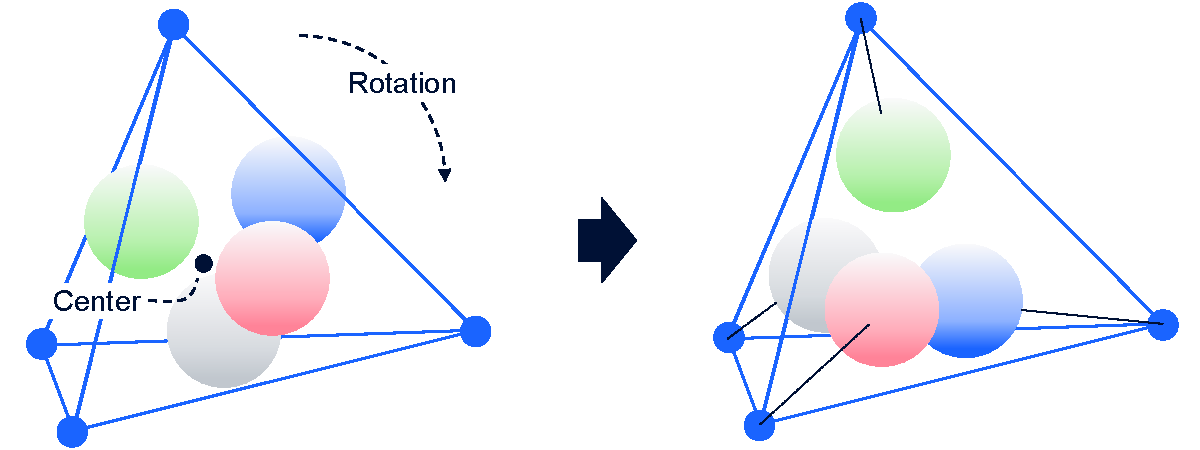
\includegraphics[width=0.8\linewidth]{figures/06_sparse_clust/init_rotate/init_rotate.pdf}
			\caption[Rotation capability required by SCA]{Illustration of the rotation of the latent representation required to best fit the simplex.}
			\label{fig:init_rotate}
		\end{figure}
		
		The problem can be illustrated from a geometrical perspective, by imagining the initial encoding layout of the ground truth classes as a structure of balls enclosed into the confined wireframe of the simplex (Fig.~\ref{fig:init_rotate}).
		A lucky initialization would have the ball-structure oriented in such a way that each ball is quite close to a vertex of the simplex, and conversely, an unlucky initialization would have balls on edges or faces of the simplex, in-between vertices.
		In case of an unlucky initialization, the sparseness loss often rips classes apart, forcing parts of a class to end up around different base points.
		In this unlucky case, the \ac{SCA} should be able to \emphnox{rotate} the encoded ball structure into a position where the balls align well with the vertices.
		However, rotations are complex operations in anything more than a few dimensions, and neural nets can not effectively realize them using the common \ac{FC} and nonlinearity layers, or their derivatives.
		In fact, neural nets which are capable of undertaking rotations, or are resistant to the rotation of input data (mostly 2-dimensional images in computer vision) are far from being available, and are actively researched \cite{rotation_invariant_1, rotation_invariant_2}.
		
		Rotating the simplex to best align with the data is also not practical, because it would break the simplicity of the calculations in the anchoring module, as well as the simple operations in the guidance module.	
		Further worsening the problem is the tied scaling of dimensions with $k$: the number of base-points used must be equal to the number of dimensions in the latent space in \ac{SCA}.
		Unfortunately, the number of parameters (the degrees of freedom) which govern rotations increase quadratically with $D$, rapidly making lucky initializations unlikely as $D$ increases. 
		Because of this, if the user wants to use more micro-clusters, the dimensionality of the latent space increases, which in turn further decreases the chance of a good initialization.
		
		I credit this behavior to the two design choices listed above: the enforcement of an internal representation/interface in a model, and the restriction of information to propagate only through this interface between parts of the model (in this case, the encoder and the decoder).
		While the representation is meant to be intuitive to us humans, it is not necessarily useful in a \ac{DL} model.
		In fact, many of the problems that are best solved today with \ac{DL} -- such as computer vision or \ac{NLP} -- were hard to solve with hand-engineered features and functions, especially because human understanding and representation does not translate well to learnable models in these tasks.
		Big breakthroughs were achieved when \ac{DL} models started to learn how to process raw data into the required output in an end-to-end fashion, instead of the then usual predefined features processed step-by-step through a chain of hard-coded or simple learned functions.
		Obviously, we have committed the same mistake in some sense with \ac{SCA}, by defining a strict internal representation that was meant to be explainable.
		Since undertaking this work, I believe that it is best to use \ac{DL} in an end-to-end fashion, feeding raw or barely processed information and implementing the solution in a single model.
		This approach minimizes human bias during design time, and allows for the \ac{DL} algorithm to learn internal representations that best suit the given model, even if these are not understandable by humans.
		
		In the case of deep clustering algorithms, the obvious solution to the above problem is to detach the cluster definitions from the internal representation, arriving at the common structure of most deep clustering methods, which utilizes a secondary clustering algorithm to define clusters in the encoding space.
		Another approach to lessen the impact of a restricted internal representation is to allow some information to pass unaffected, and only use parts of the encoding space for the given task, such as clustering.
		Both of these ideas are incorporated in the deep clustering algorithm which is discussed in the next chapter.
		
		Barring major modifications, specifically for \ac{SCA}, a solution to the initialization problem could be to pretrain the model with clusters defined in another algorithm, so that clusters are immediately mapped close to the base-points before sparsity is enforced.
		We did not evaluate this idea, because initializing a clustering algorithm with another clustering algorithm kind of defeats the purpose of having the second algorithm, however, if the goal is to create precise state-transition graphs, this could be a solution.
		As to which clustering algorithm to use to find the initial clusters, I can recommend the algorithm introduced in the next chapter, which provides excellent results on mobile network data due to its unbiased nature.
		
		In the end, deep learning models contain complex logic, which is hard to explain.
		On one hand, attempts at forcing a \ac{DL} model to have a simple, explainable representation could very well end up lowering its modeling power, or even completely destroying its capacity to model a certain problem.
		On the other hand, \ac{DL} algorithms are often not considered for critical tasks, because their internal logic is opaque, and we don't trust them.
		My hope is that in the future, with the advancement of postprocessing-based explanation techniques -- such as the ``dreams'' shown in Sec.~\ref{cha:deep_learning:sec:hierarchical_features} --  we will not need to design \ac{DL} algorithms for explainability, never compromising their complexity and thus, modeling capacity.
